\documentclass{article}
%%%%%%% PACKAGES %%%%%%%%
\usepackage[utf8]{inputenc}
\usepackage{graphicx,wrapfig,lipsum}
\usepackage{geometry}
\geometry{a4paper, margin=1in}
\usepackage{hyperref}
\usepackage{titling}
\usepackage{caption}
\usepackage{subcaption}
\usepackage{float}
\hypersetup{
    colorlinks=true,
    linkcolor=blue,
    filecolor=magenta,      
    urlcolor=blue,
}

\title{Algorithms: Design \& Analysis Project Proposal \\
        \large Optimizing the Knapsack: \\
        A Comparative Algorithm Analysis}
\author{Project Team 2}
\date{\today}

\begin{document}

\maketitle

\section*{Team}
\begin{tabular}{ l l }
    Ali Asghar Yousuf & ay06993@st.habib.edu.pk \\ 
    Aumaima Rahid & ar06173@st.habib.edu.pk \\ 
    Mohammad Haider Abbas & ma06418@st.habib.edu.pk \\
    Radhika Khatri & rk06365@st.habib.edu.pk \\
    Syed Muhammad Abbas Haider Taqvi & st06862@st.habib.edu.pk 
   \end{tabular}
\section*{Overview}
We will be solving the 0-1 Knapsack problem using different algorithms. We will implement the algorithms in \texttt{Python} and compare their results as well as their time complexity.
\section*{Background}
\begin{wrapfigure}{r}{5.5cm}
\caption{Knapsack}\label{wrap-fig:1}
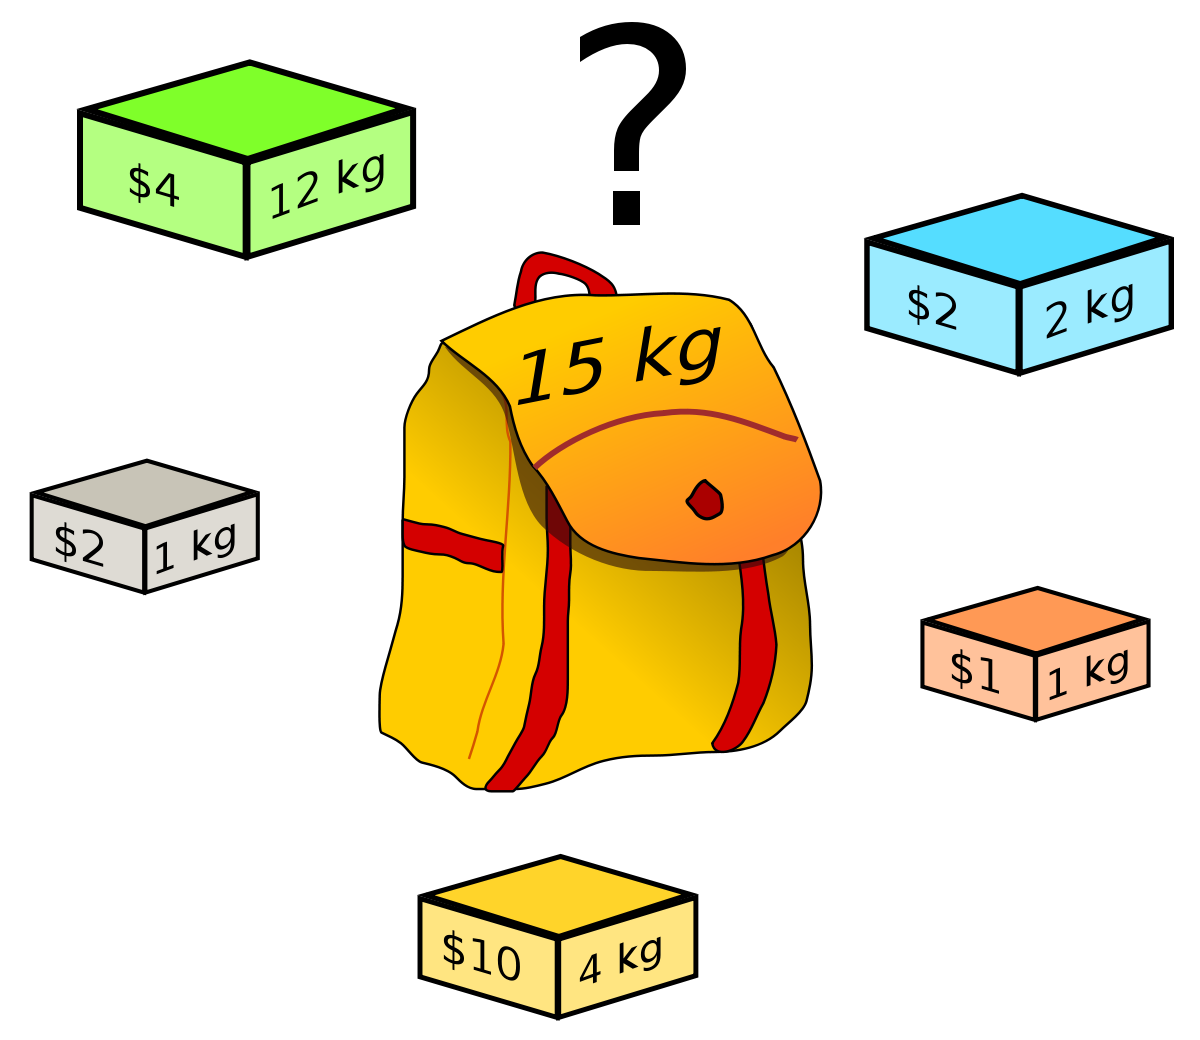
\includegraphics[width=5.5cm]{knapsack.png}
\end{wrapfigure} 
%------------------------------------------
Knapsack problem is a problem in combinatorial optimization: Given a set of items, each with a weight and a value, determine which items to include in a collection so that the total weight is less than or equal to a given limit and the total value is as large as possible.
It derives its name from the problem faced by someone who is constrained by a fixed-size knapsack and must fill it with the most valuable items. The problem often arises in resource allocation where the decision makers have to choose from a set of non-divisible projects or tasks under a fixed budget or time constraint, respectively.
It is also used in the context of computer science and operations research, where it is called the bin packing problem, and in microeconomics, where it is called the assignment problem.

There are two variants of the knapsack problem: the 0-1 knapsack problem and the unbounded knapsack problem. In the 0-1 knapsack problem, also called the discrete knapsack problem, each item can be included in the knapsack at most once. In the unbounded knapsack problem, also called the continuous knapsack problem, each item can be included in the knapsack any number of times.

\section*{Algorithms}
We will be implementing and analyzing the following algorithms:
\begin{itemize}
    \item Brute Force
    \item Greedy Algorithm
    \item Dynamic Programming
    \item Evolutionary Algorithm
\end{itemize}

\subsection*{Brute Force}
Brute force is a method of solving a problem by trying all possible solutions. It is a very general problem-solving technique that can be applied to many different types of problems. It is often used when the problem is easy to state, but difficult to solve. Brute force is a very simple algorithm, but it is not always the most efficient. It is often used as a last resort when other algorithms fail to produce a solution. Since it is computationally very expensive, it is nearly impossible to solve problems with a large number of variables. 

\subsection*{Greedy Algorithm}
Greedy algorithms are a class of algorithms that follow the problem solving heuristic of making the locally optimal choice at each stage with the hope of finding a global optimum. In many problems, a greedy strategy does not in general produce an optimal solution, but nonetheless a greedy heuristic may yield locally optimal solutions that approximate a globally optimal solution in a reasonable time.

\subsection*{Dynamic Programming}
Dynamic programming is both a mathematical optimization method and a computer programming method. The method was developed by Richard Bellman in the 1950s and has found applications in numerous fields, from aerospace engineering to economics. In both contexts it refers to simplifying a complicated problem by breaking it down into simpler sub-problems in a recursive manner. While some decision problems cannot be taken apart this way, decisions that span several points in time do often break apart recursively.
Likewise, in computer science, if a problem can be solved optimally by breaking it into sub-problems and then recursively finding the optimal solutions to the sub-problems, then it is said to have optimal substructure. A dynamic programming algorithm examines each sub-problem only once, whereas naive methods may repeat the examination of a given sub-problem many times. In computer science, dynamic programming is used in solving problems that can be broken down into optimal sub-problems.
The sub-problems are stored in a \texttt{memo}, and the solutions to the sub-problems are used to find the solution to the original problem.

\subsection*{Evolutionary Algorithm}
Evolutionary algorithms (EAs) are computational methods inspired by natural evolution, such as natural selection, genetics, and survival of the fittest. They are used to generate solutions to optimization and search problems. They are particularly useful when the search space is large and brute force methods are not feasible. They have both exploitative and explorative components. Exploitation refers to the use of current knowledge to improve the current solution, while exploration refers to the use of knowledge to search for better solutions in the search space. Which means they are better at finding global optima instead of getting stuck in local optima like in greedy algorithms.
\section*{Dataset}
We will be using the following dataset:

\begin{itemize}
    \item \href{https://people.sc.fsu.edu/~jburkardt/datasets/knapsack_01/knapsack_01.html}{Knapsack 0/1}
\end{itemize}

Note: The dataset maybe changed if we find a better one.

\section*{References}
\begin{itemize}
    \item \href{https://www.geeksforgeeks.org/0-1-knapsack-problem-dp-10/}{0-1 Knapsack Problem}
    \item \href{https://www.geeksforgeeks.org/brute-force-approach-and-its-pros-and-cons/}{Brute Force Approach}
    \item \href{https://www.geeksforgeeks.org/greedy-algorithms/}{Greedy Algorithms}
    \item \href{https://www.geeksforgeeks.org/dynamic-programming/}{Dynamic Programming}
    \item \href{https://www.sciencedirect.com/topics/mathematics/evolutionary-algorithm/}{Evolutionary Algorithm}
\end{itemize}
\end{document}